\documentclass[11pt,a4paper]{jsarticle}
%
\usepackage{amsmath,amssymb}
\usepackage{bm}
\usepackage[dvipdfmx]{graphicx}
\usepackage{ascmac}
\usepackage{listings,jvlisting} 
\usepackage{float}
%
\setlength{\textwidth}{\fullwidth}
\setlength{\textheight}{40\baselineskip}
\addtolength{\textheight}{\topskip}
\setlength{\voffset}{-0.2in}
\setlength{\topmargin}{0pt}
\setlength{\headheight}{0pt}
\setlength{\headsep}{0pt}
%
\newcommand{\divergence}{\mathrm{div}\,}  %ダイバージェンス
\newcommand{\grad}{\mathrm{grad}\,}  %グラディエント
\newcommand{\rot}{\mathrm{rot}\,}  %ローテーション
%

\lstset{
  basicstyle={\ttfamily},
  identifierstyle={\small},
  commentstyle={\smallitshape},
  keywordstyle={\small\bfseries},
  ndkeywordstyle={\small},
  stringstyle={\small\ttfamily},
  frame={tb},
  breaklines=true,
  columns=[l]{fullflexible},
  numbers=left,
  xrightmargin=0zw,
  xleftmargin=3zw,
  numberstyle={\scriptsize},
  stepnumber=1,
  numbersep=1zw,
  lineskip=-0.5ex
}

%

\title{システムソフトウェア中間課題}
\author{21B30362 佐久川泰輔}
\date{\today}
\begin{document}
\maketitle
%
%
\section{問1\_1}
\subsection{コードの説明}
以下は、スレッドライブラリを実装しているuthreads.の一部である。

\begin{lstlisting}[caption=uthreads.cの冒頭]
#define STACK_DEPTH 512
#define MAX_THREADS 4

#define UNUSED 0
#define RUNNABLE 1
#define RUNNING 2

struct uthread {
    int tid;
    int state;
    uint64 stack[STACK_DEPTH];
    struct context my_context;
    void (*fun)();
};

struct uthread uthreads[MAX_THREADS];
struct uthread *current_thread;
struct context start_context;
\end{lstlisting}

構造体uthreadは、スレッドを構成するための構造体である。

スレッドの作成を行う関数は以下である。
\begin{lstlisting}[caption=make\_uthread]
int make_uthread(void (*fun)()) {
    int empty = -1;
    for (int i = 0; i < MAX_THREADS; i++) {
        if (uthreads[i].state == UNUSED) {
            empty = i;
            break;
        }
    }
    
    if(empty == -1) {
        return -1;
    }

    struct uthread *thread = malloc(sizeof(struct uthread));
    thread->tid = empty;
    thread->state = RUNNABLE;
    thread->fun = fun;
    thread->my_context.ra = (uint64) fun;
    thread->my_context.sp = (uint64)(thread->stack + STACK_DEPTH);
    uthreads[empty] = *thread;

    return thread->tid;
}
\end{lstlisting}

まず、2-8行目で、uthreads配列のうち、空いている場所を特定する。空いている場所が無い場合、スレッドの作成を行わず-1を返す。

次に、uthread構造体を1つ作り、スレッドの初期化を行い、そのスレッド番号を返す。

\

以下は、スレッドの開始を行う関数である。
\begin{lstlisting}[caption=start\_uthread]
void start_uthreads() {
    current_thread = &uthreads[0];
    current_thread->state = RUNNING;

    start_context.ra = (uint64) start_uthreads;
    start_context.sp = (uint64)(current_thread->stack + STACK_DEPTH);
    swtch(&start_context, &current_thread->my_context);
}
\end{lstlisting}

配列の0番目をcurrent\_threadとした後にそれを実行状態にし、現在の関数の情報をstart\_conextに記録する。

その後、swtch()によりcurrent\_threadに処理を切り替える。
\
以下は、スレッドを切り替える関数yield()である。
\begin{lstlisting}[caption=yield]
void scheduler() {
    struct uthread *t = 0;
    struct uthread *prev = current_thread;
    int i;

    for (i = current_thread->tid + 1; i <= current_thread->tid + MAX_THREADS; i++) {
        if (i >= MAX_THREADS) i -= MAX_THREADS;
        if (uthreads[i].state == RUNNABLE) {
            t = &uthreads[i];
            break;
        }

        if (i == current_thread->tid) {
            swtch(&prev->my_context, &start_context);
            return;
        }
    }

    t->state = RUNNING;
    if (t != current_thread) {
        current_thread = t;
        swtch(&prev->my_context, &current_thread->my_context);
    }
}

void yield() {
    current_thread->state = RUNNABLE;
    scheduler();
}
\end{lstlisting}

関数yield()のうち、実際に処理を切り替える部分は別の関数scheduler()に抽出してある。これは、後の実装でこの部分を使いまわす事が可能になるからである。

まず、current\_threadを実行可能状態にする。

その後、uthreadsから実行可能なスレッドを一つ選択する。選択できなかった場合、そこで処理を中断する。

選択できた場合、そのスレッドを実行状態にし、current\_threadとした後で、swtch()により処理を切り替える。

\
以下は、現在実行中のスレッドIDを返す関数である。

\begin{lstlisting}[caption=mytid]
int mytid() {
    return current_thread->tid;
}
\end{lstlisting}
current\_threadのスレッド番号を返す。

\subsection{テストコードの実行}
以下は、uthreads.cのテストコードuttest1\_1.cである。ただし、include文等は省略してある。
\begin{lstlisting}[caption=uttest1\_1.cの一部]
static int hoge = 0;

void foo() {
    for (;;) {
        printf("foo (tid=%d): %d\n", mytid(), hoge);
        hoge++;
        yield();
    }
}

void bar() {
    int c = 0;
    for (;;) {
        printf("bar (tid=%d): %d\n", mytid(), hoge);
        yield();
        c++;
        hoge += c;
    }
}

int main() {
    make_uthread(foo);
    make_uthread(bar);
    start_uthreads();
    printf("main (tid=%d): end\n", mytid());
    exit(0);
}
\end{lstlisting}

これを実行した結果は以下である。
\begin{figure}[H]
  \centering
 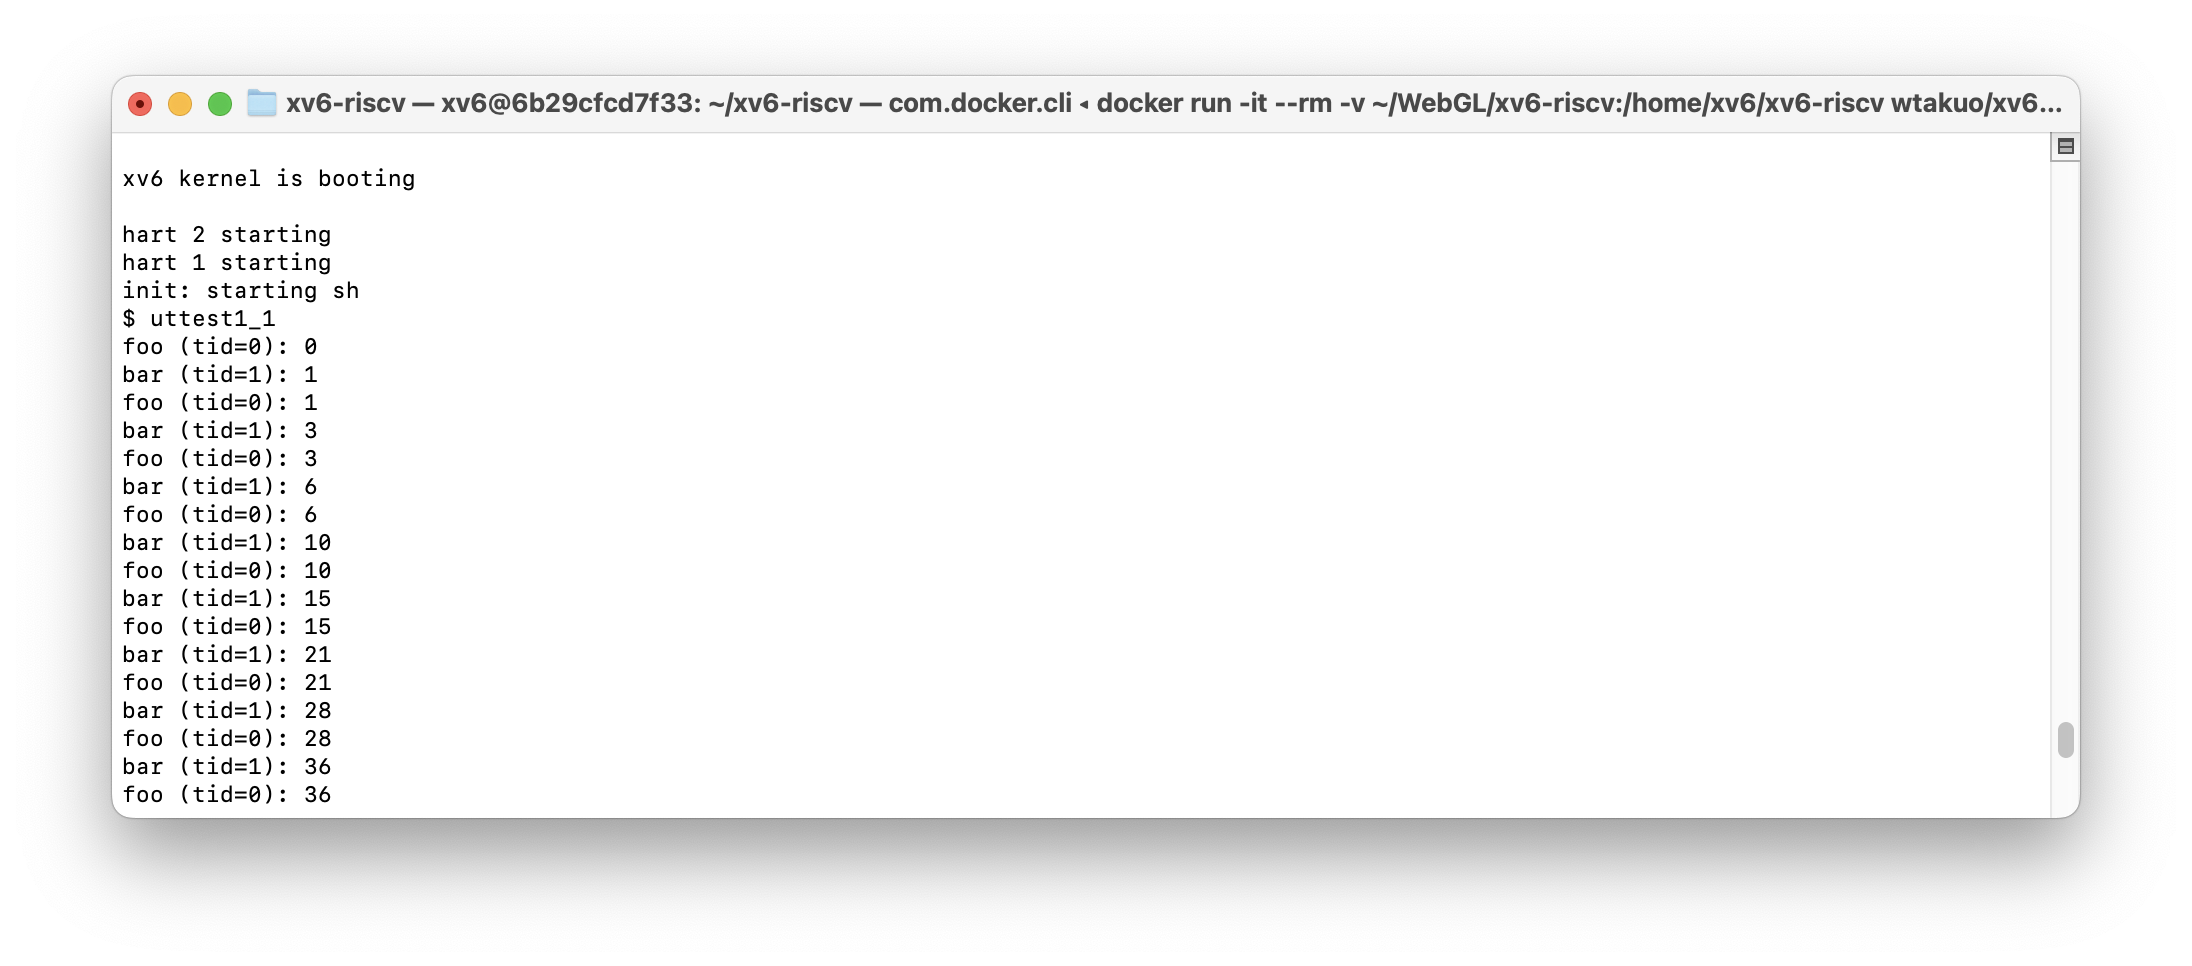
\includegraphics[width=10cm]{image/image1.png}
  \caption{uttest1\_1.cの実行結果}
\end{figure}

\section{問1\_2}
\subsection{コードの説明}
以下は、スレッドを終了させる関数uthread\_exit()である。
\begin{lstlisting}[caption=uthread\_exit]
void uthread_exit() {
    current_thread->state = UNUSED;
    free(current_thread);
    scheduler();
}
\end{lstlisting}

まず、現在のスレッドの位置を未使用状態にする。

その後、スレッドに使用していたメモリを解放する。

最後に、yield()の時と同様に別のスレッドに実行を移す。

その際に、全てのスレッドの実行が終了した場合、start\_contextとcurrent\_threadがswtch()されるため、再度start\_uthreads()から戻る。

\subsection{テストコードの実行}
以下は、uthreads.cのテストコードuttest2.cである。ただし、include文等は省略してある。
\begin{lstlisting}[caption=uttest2.cの一部]
void foo() {
    int c = 0;
    for (;;) {
        printf("foo (tid=%d): %d\n", mytid(), c);
        c += 1;
        yield();
        if (c > 6)uthread_exit();
    }
}

void bar() {
    int c = 0;
    for (;;) {
        printf("bar (tid=%d): %d\n", mytid(), c);
        yield();
        c += 2;
        if (c > 8)uthread_exit();
    }
}

void baz_sub(int *cp) {
    printf("baz (tid=%d): %d\n", mytid(), *cp);
    yield();
    *cp += 3;
}

void baz() {
    int c = 0;
    for (;;) {
        baz_sub(&c);
        baz_sub(&c);
        if (c > 10) uthread_exit();
    }
}

int main() {
    make_uthread(foo);
    make_uthread(foo);
    make_uthread(bar);
    make_uthread(baz);
    start_uthreads();
    make_uthread(bar);
    make_uthread(baz);
    start_uthreads();
    exit(0);
}
\end{lstlisting}

これを実行した結果は以下である。
\begin{figure}[H]
  \centering
 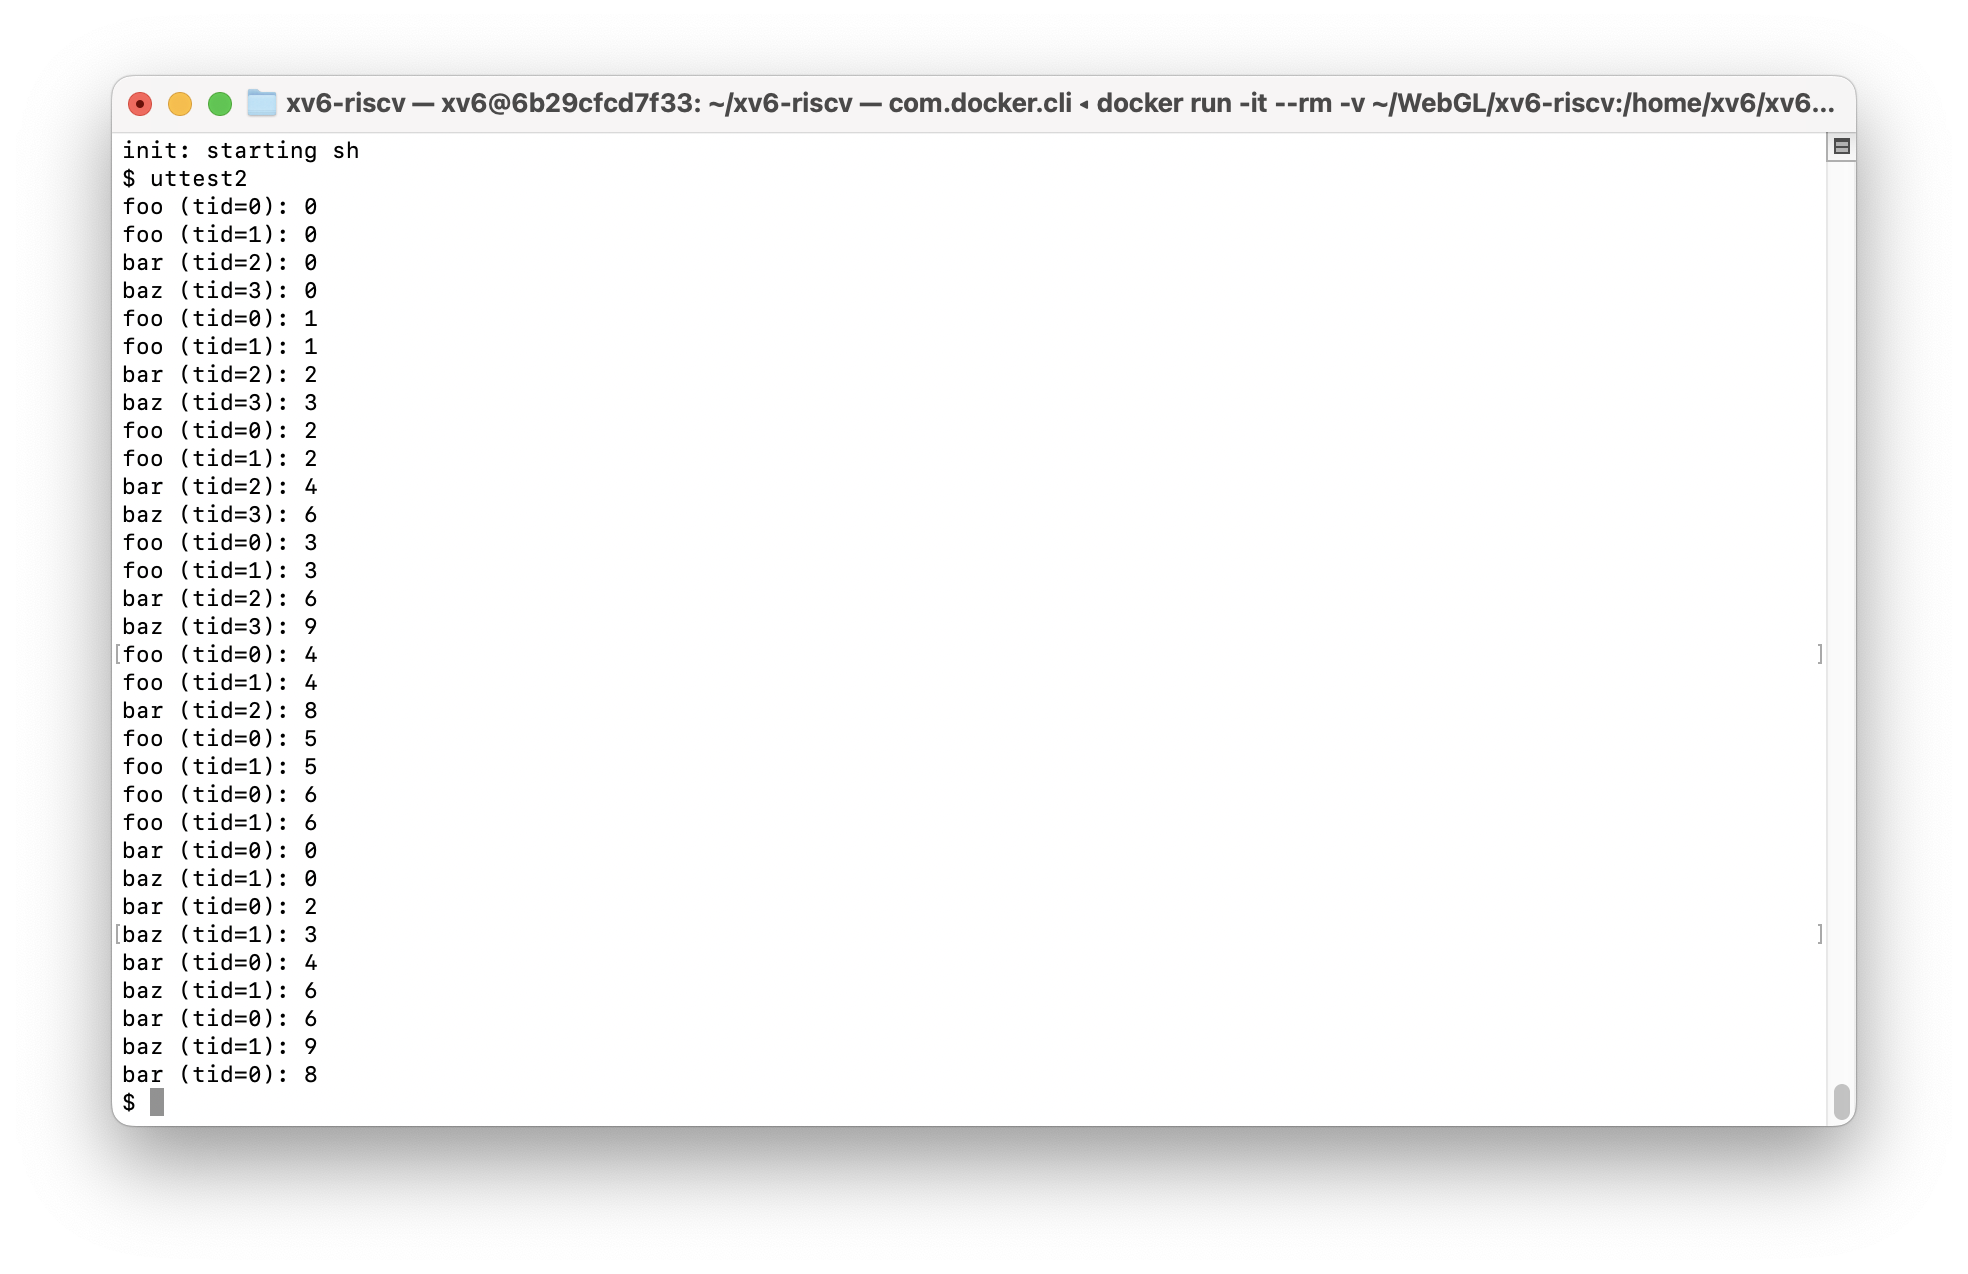
\includegraphics[width=10cm]{image/image2.png}
  \caption{uttest2.cの実行結果}
\end{figure}


\end{document}